\section{Query Answering with Routing Proxies}
\label{sec-query}

In this section, we show how to answer shortest path and distance queries using routing proxies.

\eat{%%%%%%%%
\begin{figure}[tb!]
%\vspace{-1ex}
\begin{center}
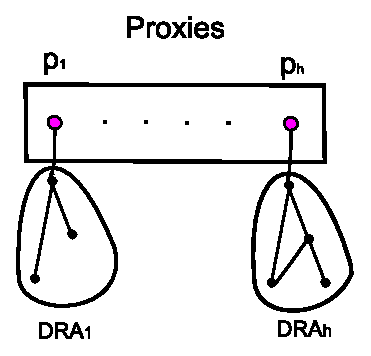
\includegraphics[scale=0.6]{./Proxy-framework.eps}
\end{center}
\vspace{-2ex}
\caption{Framework of using proxies}
\label{fig-angent-landmarks} \vspace{-2ex}
\end{figure}
}%%%%%%%%%%%%EAT

 Based on the previous analyses, we present a framework for speeding-up shortest  path and distance query answering, which consists of two modules: {\em preprocessing} and {\em query answering}.
 %The framework for answering queries using proxies and \dras is illustrated in Fig.~\ref{fig-angent-landmarks}, in which each $p_i$ ($i\in[1, h]$) denotes a proxy, and is associated with its \dra.
 We next introduce the details of the framework.

\stitle{1. Preprocessing}. Given graph $G(V, E)$, the preprocessing module executes the following.

\sstab (1) It first computes all \dras and their maximal proxies with algorithm $\compDRAs$ (to be seen shortly in Section~\ref{sec-proxy-algorithms}).

\sstab (2) It then pre-computes and stores all the shortest paths and distances between any node in a \dra and its proxy.

To support shortest distance queries, for each node in a \dra, we store its proxy $u$, its distance to $u$ and the component of $A^{+}_u$ to which it belongs,
and, moreover, to support shortest path queries, we further keep the shortest paths from proxy $u$ to all nodes in the \dra.

\sstab (3) It finally computes the reduced subgraph $G'$ by removing all \dras, but keeping their proxies, from graph $G$. 


\stitle{2. Query answering}. Given two nodes $s$ and $t$ in graph $G(V, E)$  and the pre-computed information, the query answering module executes the following.


\sstab (1) When nodes $s$ and $t$ belong to the same \dra $G[A^+_u]$ with proxy $u$ such that $A^+_u$ = $A^1_u\cup\ldots A^h_u$.

If $s$ and $t$ further fall into the same component $A^i_u$ ($i\in[1,h]$), it invokes the Dijkstra's algorithm on the subgraph $G[A^i_u]$ to compute the shortest path and distance between $s$ and $t$. Otherwise, it simply returns $\path(s, u)/\path(u, t)$ or $\dist(s, u)$ + $\dist(u, t)$ in constant time.

\sstab (2)  When $s$ and $t$ belong to two \dras $G[A^+_{u_s}]$ and $G[A^+_{u_t}]$ with proxies $u_s$ and $u_t$, respectively.

By the analyses in Section~\ref{subsec-proxy-properties}, we know that $\path(s, t)$ = $\path(s, u_s)/\path(u_s, u_t)/$ $\path(u_t, t)$, in which $\path(s, u_s)$ and $\path(u_t, t)$ are already known. Hence, it simply invokes an algorithm (\eg bidirectional Dijkstra~\cite{LubyR89}, \arcflag \cite{MohringSSWW05}, \ch~\cite{GeisbergerSSD08}, \tnr~\cite{bast2014route}, \ah~\cite{zhu2013shortest}) on the reduced graph $G'$ for computing $\path(u_s, u_t)$.

Similarly, the shortest distance $\dist(s, t)$ = $\dist(s, u_s)$ + $\dist(u_s, u_t)$ + $\dist(u_t, t)$ can be computed.

We next illustrate how shortest path and distance queries are performed  with an example below.


%%%%%%%%%%%%%%%%%%%%%%%%%%%%%%%%%%%%%%%%%%%%%%%%%%
\begin{figure}[tb!]
%\vspace{-1ex}
\begin{center}
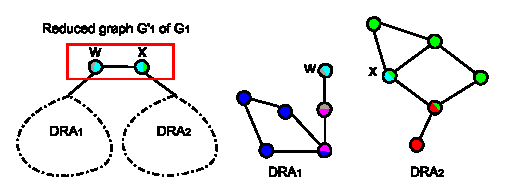
\includegraphics[scale=0.95]{./Example-framework.eps}
\end{center}
\vspace{-2ex}
\caption{Example query answering}
  \label{fig-query-answering}\vspace{-3ex}
\end{figure}

\begin{example}
\label{exm-query}
Consider graph $G_1$ and its \bccs in Fig.~\ref{fig-cut-nodes}(1), in which the \dras and their maximal proxies are computed by algorithm $\compDRAs$, \ie\ $\dra_1$ = $\{u, v, BC_1, BC_2, BC_3\}$ with its proxy $w$ and $\dra_2$ = $\{y, BC_5, BC_6\}$ with its proxy $x$, as shown in Fig.~\ref{fig-query-answering}. Note that here both $A^{+}_w$ and $A^{+}_x$ have single components. Moreover, the reduced graph $G'_1$ of $G_1$  is the subgraph with nodes $w$ and $x$ only.




\sstab(1) Consider nodes $s$ in $\dra_1$  and $t$ in $\dra_2$, we first compute $\dist(w, x)$ or $\path(w,x)$ on $G'_1$, and then 
let $\dist(s, t)$ = $\dist(s, w)$ + $\dist(w, x)$ + $\dist(x, t)$ or $\path(s, t)$ = $\path(s, w)/\path(w, x)/\path(x, t)$.
Note that here $\dist(s, w)$, $\dist(x, t)$, $\path(s, w)$ and $\path(x, t)$ have all been computed in the precessing stage.


\sstab(2) If nodes $s$ and $t$ are both in $\dra_1$  or $\dra_2$, we directly compute their shortest path or distance on  $\dra_1$  or $\dra_2$,
as they have single components.
\end{example}

\vspace{-1ex}
\stitle{Remarks}.
(1) As shown above, we need $O(d)$ extra space to store the routing information to compute shortest paths and distances, where $d$ is the total number of nodes in all \dras.

\sstab (2) It is easy to see that the main computation cost is reduced from graph $G$ to its reduced graph $G'$. As shown in the experimental study (Section~\ref{sec-expt}), on average about 1/3 nodes of a graph are captured by non-trivial proxies and their \dras, \ie $d$ is about $|V|/3$. That is, the reduced graph $G'$ is about 2/3 size of the original graph $G$, and hence our data reduction technique could reduce graph sizes and speed up shortest path and distance computations. 